\documentclass[a4paper,11pt]{article}
\usepackage{array}
\usepackage{booktabs}
\usepackage[utf8]{inputenc}
\usepackage{fontenc}
\usepackage[ngerman]{babel}
\usepackage{csquotes}
\usepackage[a4paper,lmargin={3cm},rmargin={3cm},
tmargin={3cm},bmargin = {2cm}]{geometry}
\usepackage{fancyhdr}
\usepackage{pdfpages}
\usepackage{parskip}
\usepackage{color}
\usepackage{amssymb}
\usepackage{amsthm}
\usepackage{graphicx}
\usepackage[onehalfspacing]{setspace}
\usepackage[backend=biber,style=alphabetic]{biblatex}
\usepackage{listings}
\usepackage{color}
\usepackage{float}

\definecolor{dkgreen}{rgb}{0,0.6,0}
\definecolor{gray}{rgb}{0.5,0.5,0.5}
\definecolor{mauve}{rgb}{0.58,0,0.82}

\lstset{frame=tb,
  language=Erlang,
  aboveskip=3mm,
  belowskip=3mm,
  showstringspaces=false,
  columns=flexible,
  basicstyle={\small\ttfamily},
  numbers=left,
  numberstyle=\tiny\color{gray},
  keywordstyle=\color{blue},
  commentstyle=\color{dkgreen},
  stringstyle=\color{mauve},
  breaklines=true,
  breakatwhitespace=true,
  tabsize=3
}

\addbibresource{library.bib}
\setcounter{tocdepth}{2}

\pagestyle{fancy}
\fancyhf{}
\rhead{Ausarbeitung eines kausalen Multicasts}
\lhead{Kristoffer Schaaf}
\rfoot{Page \thepage}

\newgeometry{
lmargin={0cm},rmargin={0cm},
tmargin={3cm},bmargin = {2cm}
}

\begin{document}

\begin{titlepage} % Suppresses displaying the page number on the title page and the subsequent page counts as page 1
	
\raggedleft % Right align the title page
	
\rule{1pt}{\textheight} % Vertical line
\hspace{0.05\textwidth} % Whitespace between the vertical line and title page text
\parbox[b]{0.75\textwidth}{ % Paragraph box for holding the title page text, adjust the width to move the title page left or right on the page
		
	{\Huge\bfseries BAI5 SoSe2024 \\[0.5\baselineskip] Ausarbeitung eines kausalen \\Multicasts}\\[2\baselineskip] % Title
	{\large\textit{Verteilte Systeme - gelesen von\\Prof. Dr. Christoph Klauck}}\\[4\baselineskip] % Subtitle or further description
	{\Large\textsc{Kristoffer Schaaf (2588265)}} % Author name, lower case for consistent small caps
		
	\vspace{0.5\textheight} % Whitespace between the title block and the publisher
		
	{\noindent FAKULTÄT TECHNIK UND INFORMATIK\\Department Informatik\\Hochschule für angewandte Wissenschaften Hamburg}\\[\baselineskip] % Publisher and logo
}

\end{titlepage} 

\newgeometry{
lmargin={3cm},rmargin={3cm},
tmargin={3cm},bmargin = {2cm}
}

\setlength{\headheight}{13.59999pt}
\tableofcontents
\thispagestyle{empty}

\newpage
% \begingroup
% \let\clearpage\relax
\setcounter{page}{1}


\section{Theorie}

\subsection{CBCast Algorithmus}

In einem Netzwerk laufen verschiedene Prozesse auf verschiedenen Knoten und teilen sich keinen Speicherplatz. Die Interaktion zwischen den verschiedenen Prozessen läuft soweit ausschließlich über die Weitergabe von Nachrichten und kein Prozess kennt das Verhalten anderer Prozesse \cite{CBCAST_1}. Der \textit{CBCast} (Chain-Based Broadcast) Algorithmus ist ein Algorithmus der im Bereich der verteilten Systeme zum Einsatz kommt und eine Lösung für genau diese Prozessinteraktion implementiert. Genutzt wie zum Beispiel vom ISIS Projekt \cite{isis_project} hat er sich in der Vergangenheit bereits mehrfach renommiert.

\begin{figure}[htbp]
\begin{center}
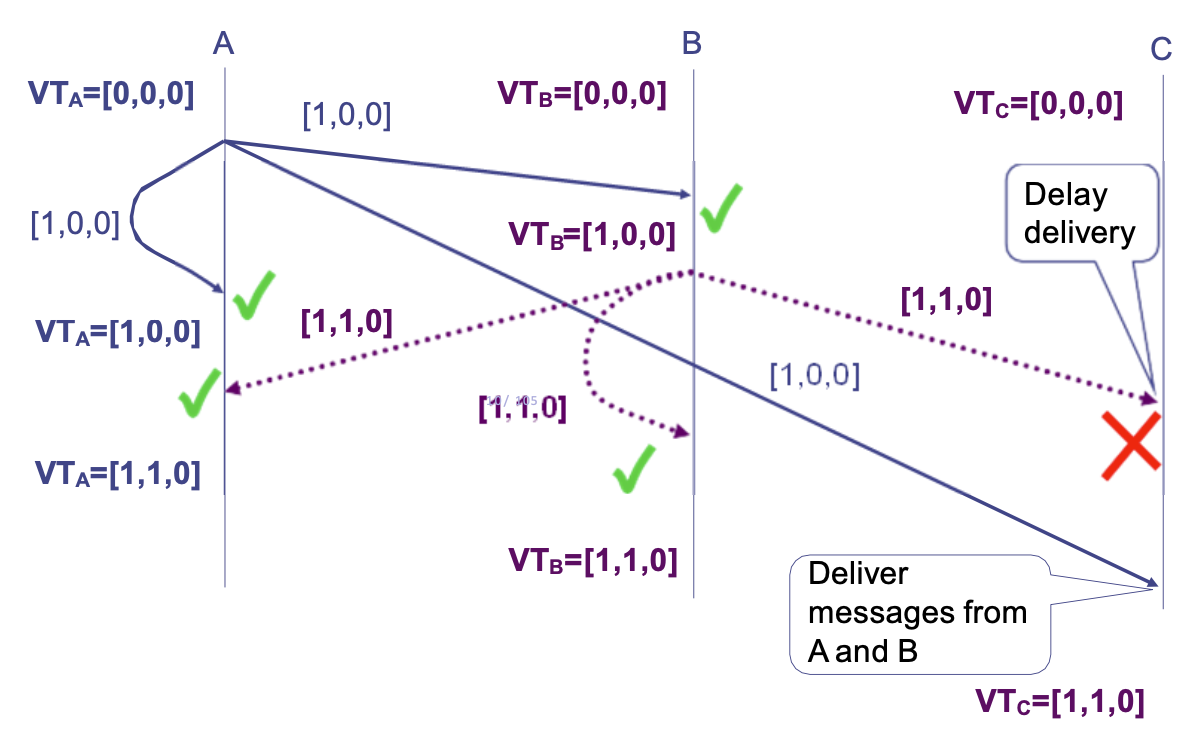
\includegraphics[scale=0.4]{Latex/Bilder/cbcast_1.png}
\caption{\label{fig:cbcastFunction} CBCAST \cite{Aufgabenstellung}} 
\end{center}
\end{figure}

In Abb. \ref{fig:cbcastFunction} zu sehen ist ein beispielhafter Ablauf des \textit{CBCASTs} mit drei Prozessen \textit{A}, \textit{B} und \textit{C}. VT zeigt die Vektoruhren der jeweiligen Prozesse. Hier wird der eigene Zeitstempel und der der anderen Prozesse individuell gespeichert. Durch diese Uhr können die Prozesse trotz fehlendem geteilten Speicherplatz erkennen, ob sie mit den anderen Prozessen synchronisiert sind.\\
Im ersten Schritt verschickt \textit{A} eine Nachricht an alle Teilnehmer im Netzwerk. Angehängt wird die eigene Vektoruhr - nun mit \textit{A} = 1 erhöht, da dieser Prozess die Nachricht verschickt hat. Wichtig hierbei ist, dass der sendende Prozess die Nachricht immer zusätzlich an sich selber schickt, um eine sichere Synchronisation sicherstellen zu können. In Abb. \ref{fig:cbcastFunction} empfangen Prozess \textit{A} und \textit{B} nun die von \textit{A} gesendete Nachricht. Die Vektoruhren werden verglichen und da jeweils nur ein Zeiger um 1 erhöht wurde, nehmen die Prozesse die gesendete Nachricht an. Nachdem \textit{B} die Nachricht von \textit{A} empfangen hat, schickt auch dieser Prozess eine Nachricht an alle Teilnehmer. \textit{A} und \textit{B} können diese empfangen. Beim Vergleichen der Vektoruhr von \textit{C} und der von \textit{B} mitgeschickten ist aber nun eine zu große Differenz. Zwei Zeiger sind jeweils um 1 erhöht, da \textit{B} bereits die Nachricht von \textit{A} empfangen hat. Bei \textit{C} fehlt diese noch, deshalb blockiert \textit{C}. Die Nachricht von \textit{A} welche daraufhin eintrifft nimmt \textit{C} dann an.\\
Die Zeiger in den Vektoruhren sind in vielen Implementierungen Zeitstempel der zuletzt empfangenen Nachricht.

\subsection{Kommunikationseinheit}

Die Kommunikationseinheit ermöglicht es Prozessen, welche über einen \textit{Tower} mit anderen Prozessen kommunizieren, Nachrichten zu schicken und zu empfangen. Das Interface stellt hierbei verschiedene Funktionen zum blockierenden und nicht blockierenden Senden von Nachrichten. Jeder Prozess, welcher als Kommunikationseinheit gestartet wird, empfängt bei korrekter Implementierung automatisch Nachrichten.

\subsubsection{Holdback Queue}

Beim Empfangen einer Nachricht, wird diese zuerst in eine \textit{Holdbackqueue} sortiert. Die \textit{Holdbackqueue} ist eine \textit{Priorityqueue} und enthält alle Nachrichten, die nicht ausgeliefert werden dürfen. Sortiert wird anhand der, der Nachricht angehängten, Vektoruhr.
\\Ob Nachrichten auslieferbar sind und die Queue verlassen dürfen oder ob Nachrichten aus der Queue gelöscht werden müssen, wird geprüft, wenn neue Nachrichten der Queue hinzugefügt werden. Falls es zu einem Stillstand im System kommt läuft zusätzlich ein Intervall-Timer, welcher die Auslieferbarkeitsprüfung regelmäßig aufruft.
\\Aus der Queue gelöscht werden, müssen Nachrichten welche %TODO

\subsubsection{Delivery Queue}

Die \textit{Deliveryqueue} ist die zweite Queue eines Kommunikationsprozesses. Sie enthält alle auslieferbaren Nachrichten und hat eine eigene Vektoruhr. Diese Vektoruhr wird synchronisiert mit jeder Vektoruhr einer, in der \textit{Deliveryqueue} neu hinzugefügten, Nachricht. 

\subsection{Vektoruhr-ADT}

Die Vektoruhr (\textit{vectorC}) wird in dieser Ausarbeitung als ein abstrakter Datentyp implementiert. Jeder Prozess hat seine eigene Vektoruhr \textit{VT}. Um eine Identität und einen initialen Zeitstempel zu erhalten, muss sich jede Vektoruhr beim Tower (Kap. \ref{tower}) melden.

\subsection{Vektoruhr Zentrale/Tower} \label{tower}

Die zentrale Vektoruhr (\textit{Tower}) verwaltet die Prozessnummern. Prozessnummern sind im Folgenden eindeutige IDs aus positiven ganzen Zahlen.

\subsection{Ungeordneter Multicast}

Ein Multicast verteilt Nachrichten an Teilnehmer in einem Netzwerk. Der Unterschied zum Broadcast besteht darin, dass beim Broadcast Inhalte verbreitet werden, die – mit geeigneter Empfangsausrüstung – jeder ansehen kann, wohingegen beim Multicast vorher eine Anmeldung beim Sender erforderlich ist \cite{wiki:Multicast}.\\
Der TowerCBC (siehe Abb. \ref{fig:towerCBC}) übernimmt in dieser Ausarbeitung die Aufgabe des ungeordneten Multicasts. Ungeordnet ist dieser, weil die Nachrichten nicht in der Reihenfolge weitergegeben werden, in der sich die jeweiligen Teilnehmer/Prozesse beim TowerCBC registriert haben.

\begin{figure}[htbp]
\begin{center}
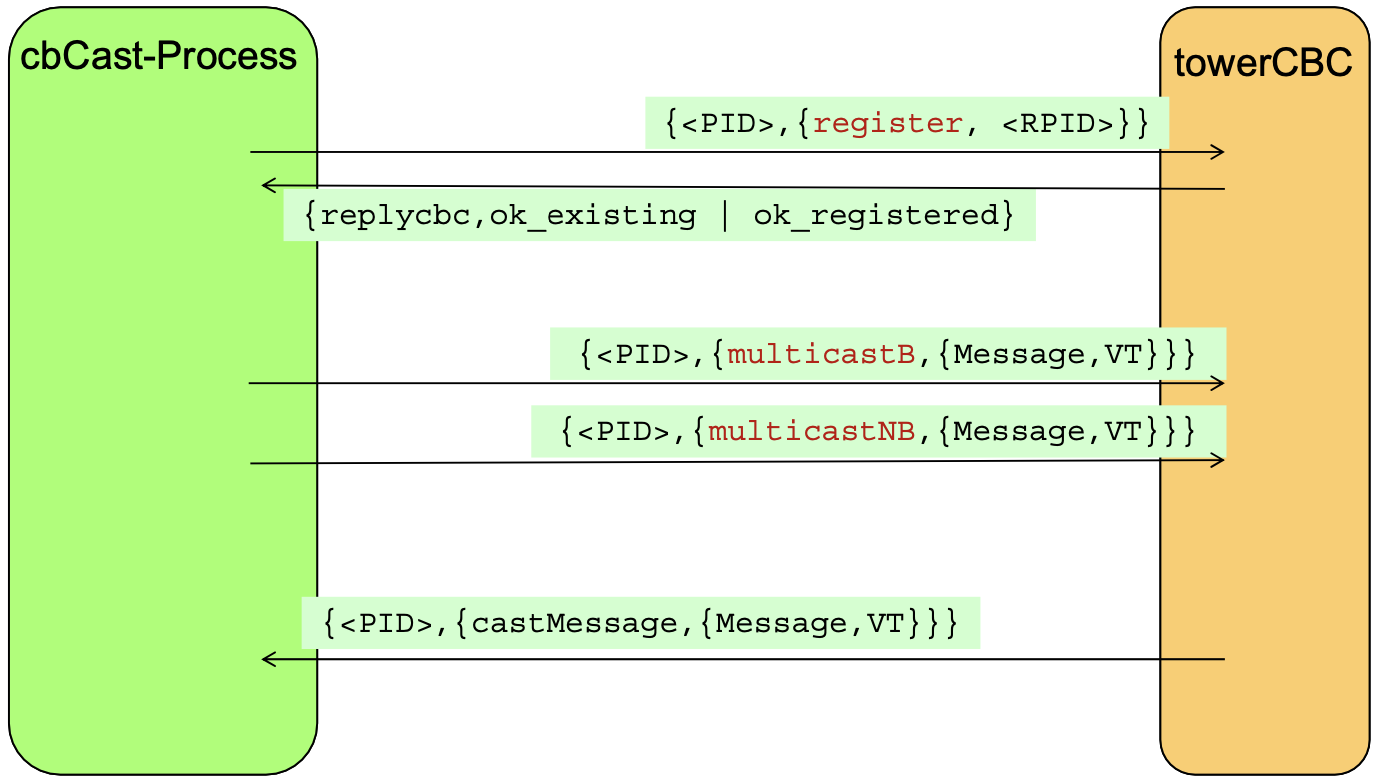
\includegraphics[scale=0.4]{Latex/Bilder/towerCBC_1.png}
\caption{\label{fig:towerCBC} ungeordneter Multicast \cite{Aufgabenstellung}} 
\end{center}
\end{figure}

In Abb. \ref{fig:towerCBC} ist eine abstrakte Kommunikation eines Prozesses mit dem Multicast dargestellt. Über \textit{register} meldet sich der \textit{cbCast-Prozess} beim \textit{towerCBC} an. Dieser bestätigt die Anmeldung. Über \textit{multicastB (blockierend)} oder \textit{multicastNB (nicht blockierend)} kann der Prozess nun Nachrichten über den Multicast an alle Teilnehmer im Netzwerk schicken. Der Multicast wieder kann mit \textit{castMessage} Nachrichten an die Teilnehmer schicken.

\subsection{Aufgabenstellung}


Fragen:

- vektorclock zählt prozesse hoch -> auf überlauf des zählers achten
- towercbc -> auto oder manu
    - bei manu empfängt der tower nur nachrichten. Aufrufe nur manuell von außen möglich
    - bei auto entscheidet tower selbst wann er welche nachrichten rausschickt. Schickt z.b. direkt raus.
- blocking/nonblocking: im manuellen zustand kann nur einer der beiden verwendet werden.
- 


Infos von Klauck aus der VL heute:

1) Eine Nachricht verlässt die dlq wenn der anwender an entsprechender comm einheit die funktion read oder receive aufruft.

2) Eine dlq hat eine eigene vektoruhr

3) Beim send vom anwender schickt dieser seine Vektoruhr mit und die Nachricht wird in hbq der anderen comm  module einsortiert und eventuell verglichen mit der vektoruhr der dlq. (siehe Bild) 

4) Beim sendeereignis tickt die uhr des anwenders.
wenn sende und empfangsereignisse in der Reihenfolge unklar sein könnten, dann müsste auch beim empfangsereignis getickt werden (Bei uns aber nicht)

5) im cbcast.erl steht das tick() im send() (zuerst)!

6) bei read und received wird sync aufgerufen (für uhr des anwenders) und ggf. auch in der dql

7) dlq kann auch länge 1 haben, macht er aber nicht so

8) wenn dlq leer ist und hbq hat lieferbare nachricht, dann sollte diese direkt in die dlq ohne das irgendwas von außen kommt - durch z.B. regelmäßige zeitliche prüfungen

9) Empfehlung von ihm: nachrichten mit after und beforeVT in HBQ einsortieren
wenn concurrent, dann müssen alle geprüft werden (Wenn der vordere nicht rüberdarf, dann die danach ziemlich sicher auch nicht)

\section{Entwurf}

\subsection{Kommunikationseinheit} \label{commModule}

\subsubsection{init/0}

Beim Initialisieren einer Kommunikationseinheit wird ein Prozess gestartet, welcher beim \textit{towerCBC} registriert wird und bei der \textit{towerClock} eine neue Vektoruhr ID anfragt. Wie in Abb. \ref{fig:sequence_cbCast_init} zu sehen, wird der Aufruf an die \textit{towerClock} von dem Prozess gesendet, der auch beim \textit{towerCBC} registriert wird. Grund dafür ist, dass die \textit{towerClock} die Prozess ID des anfragenden Prozesses auf dessen Vektoruhr ID mappt. Würde der Prozess, welcher den \textit{cbCast} Prozess erzeugt diese Anfrage schicken, würde dieses Mapping eine falsche Prozess ID speichern.
\\Der Verbindungsaufbau oder auch Verbindungstest terminiert das Programm, wenn er fehlschlägt.
\\Nach Erzeugung des \textit{cbCast} Prozesses ist dieser sequenziell nicht mehr gebunden an den Prozess, der diesen erzeugt hat. Dementsprechend verlaufen die Aufrufe dieser beiden Nebenläufig.

\begin{figure}[htbp]
\begin{center}
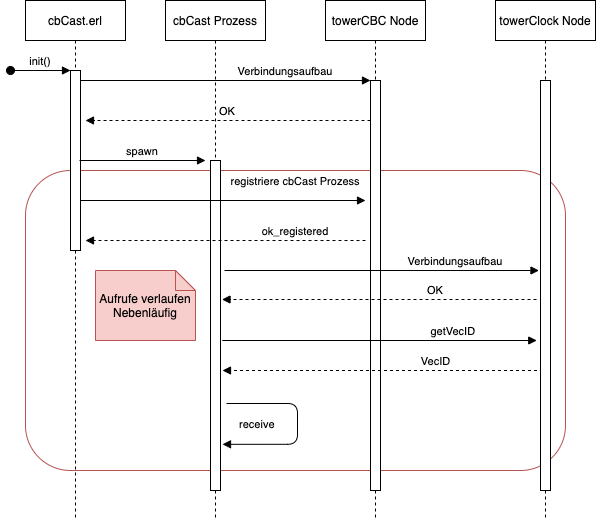
\includegraphics[scale=0.55]{Latex/Bilder/Sequenzdiagramm_cbCast.png}
\caption{\label{fig:sequence_cbCast_init} Sequenzdiagramm Initialisierung}
\end{center}
\end{figure}

Alternativ könnte sich der \textit{cbCast.erl} auch erst beim \textit{towerClock} die \textit{VektorID} holen und dann den \textit{cbCast} Prozess erzeugen. Durch den Ablauf in Abb. \ref{fig:sequence_cbCast_init} kann das holen der \textit{VektorID} aber nebenläufig zur Registrierung beim \textit{towerCBC} passieren. Der ganze Vorgang ist somit schneller.

\subsubsection{stop/1}

Die Terminierung erfolgt auf zwei verschiedene Wege. Zuerst wird der Prozess gestoppt, das bedeutet das eine sogenannter \textit{Graceful Shutdown} durchgeführt wird. Hat dieser kein Erfolg wird der Prozess durch einen \textit{Hard Shutdown} gekillt.\\
Als Parameter wird der zu terminierende Prozess übergeben.

\subsubsection{send/2}

Beim Senden (siehe Abb. \ref{fig:sequence_cbCast_send}) wird eine Nachricht \textit{(Msg)} an den als Parameter übergebenen \textit{Kommunikationsprozess (cbCast Prozess)} geschickt. Dieser erhöht seine Vektoruhr vor dem Senden um 1 und verschickt die Nachricht an den \textit{Multicast}. Der \textit{Multicast} verteilt die Nachricht an alle Prozesse, inklusive dem Sender.\\
Die Vektoruhr der versendeten Nachricht hat zu der Vektoruhr der \textit{Kommunikationseinheit} eine Distanz von -1, wodurch diese Nachricht auslieferbar ist und direkt in die \textit{Delivery Queue} einsortiert werden könnte.
Wenn die gesendete Nachricht vom \textit{Multicast} empfangen wird, wird diese dennoch zuerst in die \textit{Holdback Queue} einsortiert um eine kausale Ordnung zu garantieren.

\begin{figure}[htbp]
\begin{center}
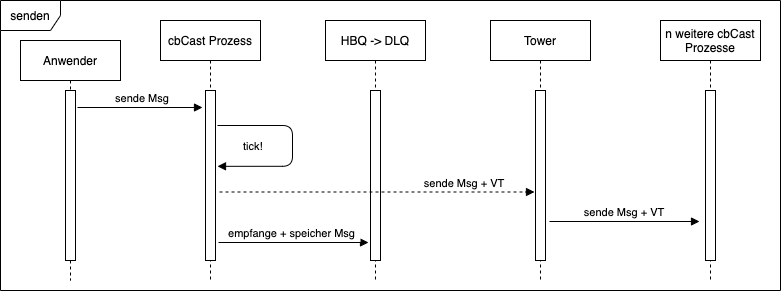
\includegraphics[scale=0.5]{Latex/Bilder/Sequenz_senden.png}
\caption{\label{fig:sequence_cbCast_send} Sequenzdiagramm Senden}
\end{center}
\end{figure}

\subsubsection{read/1 \& received/1}

\begin{figure}[htbp]
\begin{center}
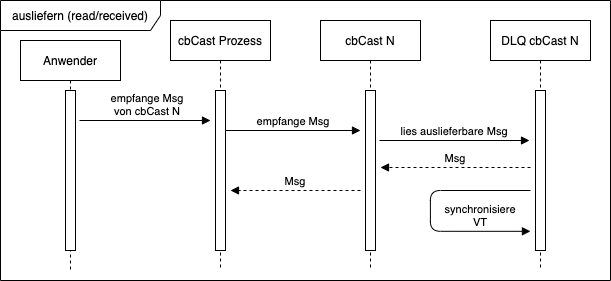
\includegraphics[scale=0.5]{Latex/Bilder/Sequenz_ausliefern.png}
\caption{\label{fig:sequence_cbCast_read_receive} Sequenzdiagramm Ausliefern}
\end{center}
\end{figure}

Das Ausliefern einer Nachrichten (siehe Abb. \ref{fig:sequence_cbCast_read_receive}) liest eine Nachricht aus der \textit{Delivery Queue} des \textit{Kommunikationsprozesses (cbCast N)}, welcher als Parameter übergeben wurde.\\
Hierfür gibt es eine Funktion, welche blockierend und eine, welche nicht blockierend empfängt.

\paragraph{read/1 (nicht blockierend)}

Falls der angefragte Prozess keine auslieferbare Nachricht zur Verfügung hat, wird nichts empfangen und der anfragende Prozess läuft normal weiter.

\paragraph{receive/1 (blockierend)}

Falls der angefragte Prozess keine auslieferbare Nachricht zur Verfügung hat, wartet der anfragende Prozess so lange, bis eine auslieferbare Nachricht empfangen wird.\\

In beiden Funktionen synchronisiert der angefragte Prozess anschließend seine Vektoruhr mit der der ausgelieferten Nachricht, falls eine Nachricht verschickt wurde.

\subsubsection{$\{\langle PID \rangle,\{castMessage,\{\langle Message \rangle, \langle VT \rangle\}\}\}$}

Wenn der \textit{Multicast (Tower)} eine Nachricht verschickt, wird diese von der Schnittstelle $\{\langle PID \rangle,\{castMessage,\{\langle Message \rangle, \langle VT \rangle\}\}\}$ der \textit{Kommunikationsprozesses} empfangen (siehe Abb. \ref{fig:sequence_cbCast_cbcast}). Daraufhin wird die Nachricht in der \textit{Holdback Queue} des Prozesses einsortiert.

\begin{figure}[htbp]
\begin{center}
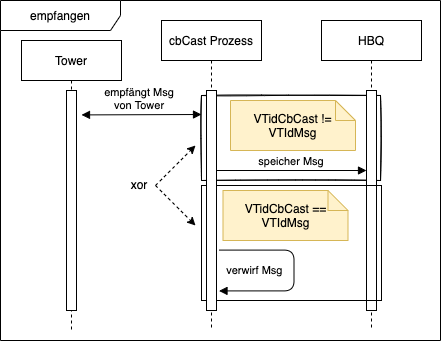
\includegraphics[scale=0.5]{Latex/Bilder/Sequenz_empfangen.png}
\caption{\label{fig:sequence_cbCast_cbcast} Sequenzdiagramm Empfangen}
\end{center}
\end{figure}

\subsubsection{Die Queues}

Sowohl die \textit{Holdback} als auch die \textit{Delivery Queue} sind Listen, welche die Nachrichten als Elemente enthalten. In der \textit{Holdback Queue} werden die Nachrichten absteigend nach den Vektoruhren der jeweiligen Nachrichten sortiert. Ist eine Nachricht \textit{after} (siehe \ref{positionVTs}) der ersten Nachricht der \textit{Holdback Queue} wird diese am Anfang einsortiert. Ist die Nachricht \textit{before} wird sie weiter mit den absteigenden Nachrichten verglichen, bis entweder das Ende der \textit{Queue} erreicht wurde oder bis die Nachricht wieder \textit{before} der an dem Index verglichenen Nachricht ist. Wenn eine Nachricht während des Einsortierens \textit{concurrent} zu einer Nachricht ist, wird sie vor dieser Nachricht einsortiert. Ist eine Nachricht \textit{equal} zu einer Nachricht in der \textit{Holdback Queue} wird sie verworfen.

\paragraph{checkQueues/3}

TODO!

\subsection{Vektoruhr-ADT}

\subsubsection{initVT/0}

\subsubsection{myVTid/1}

\subsubsection{myVTvc/1}

\subsubsection{myCount/1}

\subsubsection{foCount/2}

\subsubsection{isVT/1}

\subsubsection{syncVT/2}

\subsubsection{tickVT/1}

\subsubsection{compVT/2}

\subsubsection{aftereqVTJ/2}

\subsection{Vektoruhr Zentrale/Tower} \label{tower}

Die zentrale Vektoruhr (\textit{Tower}) verwaltet die Prozessnummern. Prozessnummern sind im Folgenden eindeutige IDs aus positiven ganzen Zahlen.

\subsection{TowerClock}

Der TowerClock implementiert eine wesentliche Schnittstelle, \textit{getVecID}. Aus Gründen der Erweiterbarkeit und Sicherheit mappt die TowerClock die Prozess ID des anfragenden Prozesses auf dessen Vektoruhr ID.
\\Die kleinste Zahl für eine Vektoruhr ID ist 0.

\subsection{Generelle Designentscheidungen}

\subsubsection{Logging}

Es wird pro Node eine generische .log Datei geben. Zum Beispiel für den Node \textit{'cbCast1@MacBook-Air-von-Kristoffer'} gibt es die Datei \textit{'cbCast1@MacBook-Air-von-Kristoffer'.log}. Dies bringt den Vorteil, dass die verschiedenen Kommunikationseinheiten - welche über die gleiche .beam Datei ausgeführt werden, aber auf verschiedenen Nodes laufen - separat voneinander geloggt werden.
\\Zum Debuggen war ein Gedanke, zusätzlich eine Logging Datei zu erstellen, in welcher alle Prozesse loggen. Hierdurch kann sequenziell nachverfolgt werden, ob die Reihenfolge der Aufrufe korrekt verläuft. Im Verlauf der Implementierung hat sich rausgestellt, dass diese Datei wenig Mehrwert bringt. Deswegen fehlt diese in der finalen Implementierung.
\section{Realisierung}

\subsection{Allgemeines}

\subsubsection{Timeouts}

In der Implementierung ist für jeden \textit{receive} Block ein \textit{Timeout} eingebaut. Dieser beträgt 1000ms. Wird der Timeout ausgelöst, wird eine für jeden Fall individuelle Fehlermeldung geloggt.

\subsubsection{Responses}

Um die jeweiligen Nachrichten und vor allem die Responses korrekt einordnen zu können, sind diese wie folgt aufgebaut:\\
Wird die Nachricht $\{self(), \{getMessage\}\}$ an den \textit{Prozess der Kommunikationseinheit} geschickt, dann ist die Antwort: $\{replycbcast, ok\_getMessage, \{...\}\}$. Anhand folgender Tabelle \ref{tab:namenszuordnung} kann eine Antwort-Nachricht eindeutig zugeordnet werden.

\begin{table}[h]
    \centering
    \begin{tabular}{|c|c|}
        \hline
        TowerClock & replyclock \\
        \hline
        TowerCBC & replycbc \\
        \hline
        Prozess der Kommunikationseinheit & replycbcast \\
        \hline
        Prozess der Queues & replyqueues \\
        \hline
    \end{tabular}
    \caption{Namenszuordnung}
    \label{tab:namenszuordnung}
\end{table}
\subsection{Kommunikationseinheit}

\subsubsection{init/0} \label{cbcast_init_realisierung}

Die Initialisierung der \textit{Kommunikationseinheit} erzeugt einen Prozess, dessen Prozess ID zurückgegeben wird.
Wie in Abb. \ref{fig:sequence_cbCast_cbcast} zu sehen muss erst eine Verbindung zum \textit{Tower} hergestellt werden. Über die \textit{erlang} Funktion \textit{net\_adm:ping/1} wird angefragt, ob die \textit{Node} des \textit{Towers} erreichbar ist. Anschließend wird der eigentlich Prozess gestartet, diesem werden zuerst die Datei, in welcher geloggt wird und die Adresse des \textit{Towers} mitgebenen.\\Aus dem neuen Prozess heraus, werden jetzt zwei wichtige Schritte getriggert:

\paragraph{Die Initialisierung der Vektoruhr} und die anschließenende Erzeugung eines neuen Prozesses für die \textit{Holdback} und \textit{Delivery Queue}, im Folgenden bezeichnet als der \textit{Prozess für die Queues}. Folgende Funktion zeigt die gespeicherten Zustände dieses Prozesses und die verfügbaren Schnittstellen.

\begin{lstlisting}
loopQueues(Datei, VT, HBQ, DLQ) ->
    receive
        {From, {pushHBQ, {Message, NewVT}}} ->
            ...
        {From, {pushDLQ, {Message, NewVT}}} ->
            ...
        {From, {popDLQ}} ->
            ...
        {From, {checkQueues}} ->
            ...
        {From, {syncVT, {AsyncVT}}} ->
            ...
        {From, {tickVT}} -> 
            ...
        {From, {getVTid}} ->
            ...
        {From, {listQueues}} ->
            ...
        Any -> 
            ...
    end.
\end{lstlisting}

Der Prozess speichert die Datei, in welcher geloggt wird als Zeichenkette, den Vektorzeitstempel in der in Kapitel \ref{vectorC_realisierung} festgelegten Datenstruktur und die \textit{Holdback} und die \textit{Delivery} Queue jeweils als Liste. Während \textit{listQueues} nur eine convenience Schnittstelle ist, welche ausschließlich zum Debuggen genutzt wird, haben alle anderen Schnittstellen eine wichtige Funktionalität: 
\begin{itemize}
    \item \textit{pushHBQ} und \textit{pushDLQ} fügen Nachrichten der jeweiligen \textit{Queue} hinzu
    \item \textit{popDLQ} entfernt eine Nachricht nach dem FiFo Prinzip aus der \textit{Delivery Queue}
    \item \textit{checkQueues} (siehe Abb. \ref{fig:flow_checkQueues}) prüft ob in der \textit{Holdback Queue} auslieferbare Nachrichten enthalten sind und sortiert diese entsprechend in die \textit{Delivery Queue}
    \item \textit{syncVT} synchronisiert die im Prozess gespeicherte Vektoruhr mit einer mitgelieferten
    \item \textit{tickVT} erhöht die im Prozess gespeicherte Vektoruhr um 1
    \item \textit{getVTid} gibt die eigene Identität der im Prozess gespeicherten Vektoruhr zurück. 
\end{itemize}

\begin{figure}[htbp]
\begin{center}
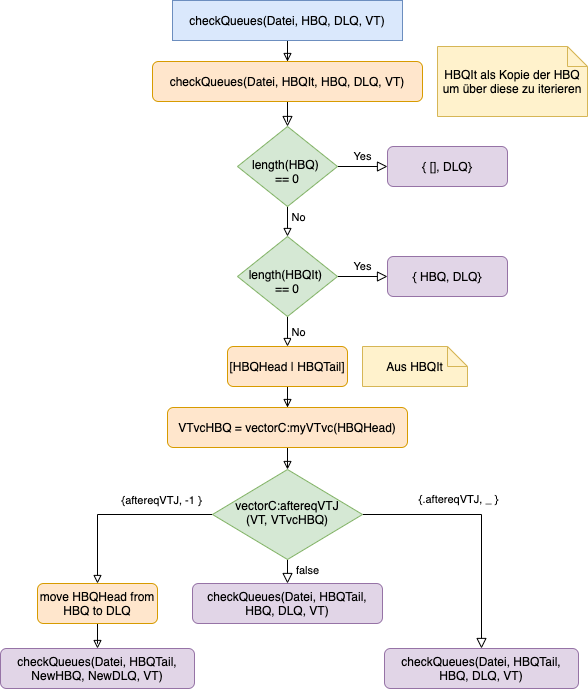
\includegraphics[scale=0.6]{Latex/Bilder/checkQueues.png}
\caption{\label{fig:flow_checkQueues} checkQueues}
\end{center}
\end{figure}
    
\paragraph{Das Empfangen von Nachrichten der Kommunikationseinheit} was das Senden und das blockierende und nicht blockierende Empfangen von Nachrichten vom und an den \textit{Tower} ermöglicht. Dieser Prozess speichert die in die zu loggende Datei, die Adresse des \textit{Towers} und die Adresse des Prozesses in welchem die \textit{Queues} gespeichert sind. Im Folgenden ist dies der \textit{Prozess der Kommunikationseinheit}.

\begin{lstlisting}
loop(Datei, TowerCBC, Queues) ->
    receive
        {_From, {castMessage, {Message, NewVT}}} ->
            ...
            loop(Datei, TowerCBC, Queues);
        ...
    end.
\end{lstlisting}

\subsubsection{stop/1} \label{cbcast_stop_realisierung}

Wie bereits in Kapitel \ref{commModule_stop} beschrieben, wird das Stoppen zuerst durch einen \textit{Graceful Shutdown} versucht. Dieser schickt eine Nachricht an den Prozess nach dessen Bearbeitung dieser sich selbst nicht wieder aufruft und somit terminiert. Schlägt dies fehl, wird nach einem Timeout die \textit{erlang} Funktion \textit{exit/2} aufgerufen und ein \textit{Hard Shutdown} durchgeführt.

\subsubsection{send/2}

Versendet wird eine Nachricht indem diese an den \textit{Prozess der Kommunikationseinheit} (\textit{cbCast Prozess}) geschickt wird (siehe Abb. \ref{fig:sequence_send_realisierung}).

\begin{figure}[htbp]
\begin{center}
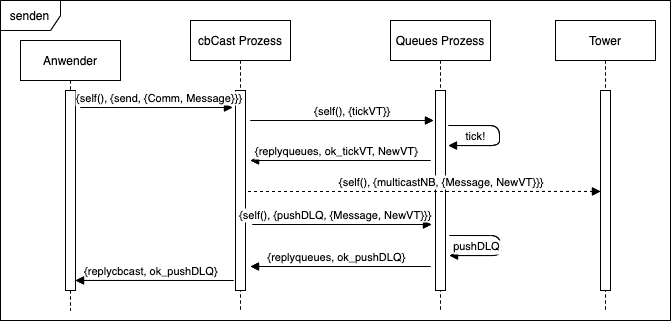
\includegraphics[scale=0.6]{Latex/Bilder/send_realisierung.png}
\caption{\label{fig:sequence_send_realisierung} send/2}
\end{center}
\end{figure}

\subsubsection{read/1 \& received/1}

Um eine Nachricht auszuliefern wird auch hier der \textit{Prozess der Kommunikationseinheit} (\textit{cbCast Prozess}) angesprochen. Beide Arten der Auslieferung schicken an die gleiche Schnittstelle. Die fragt dann über den mitgeschickten Parameter \textit{Blocking} ab ob blockierend oder nicht blockierend ausgeliefert werden soll.

\paragraph{read/1 (nicht blockierend)}

Das nicht blockierende Ausliefern schickt die Nachricht $\{self(), \{getMessage, false\}\}$ (siehe Abb. \ref{fig:sequence_read_realisierung}).

\begin{figure}[htbp]
\begin{center}
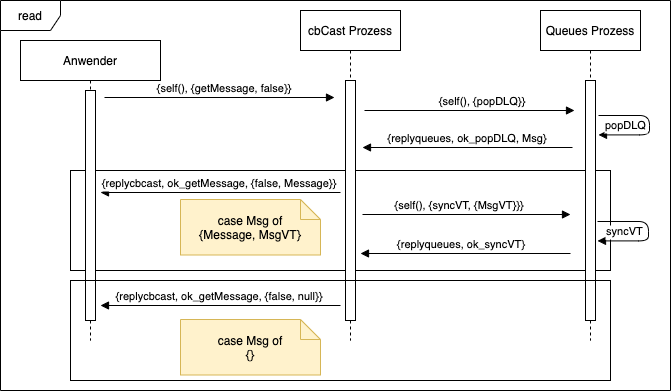
\includegraphics[scale=0.6]{Latex/Bilder/read_realisierung.png}
\caption{\label{fig:sequence_read_realisierung} read/2}
\end{center}
\end{figure}

\paragraph{received/1 (blockierend)}

Das blockierende Ausliefern schickt die Nachricht \\$\{self(), \{getMessage, true\}\}$ (siehe Abb. \ref{fig:sequence_received_realisierung}).

\begin{figure}[htbp]
\begin{center}
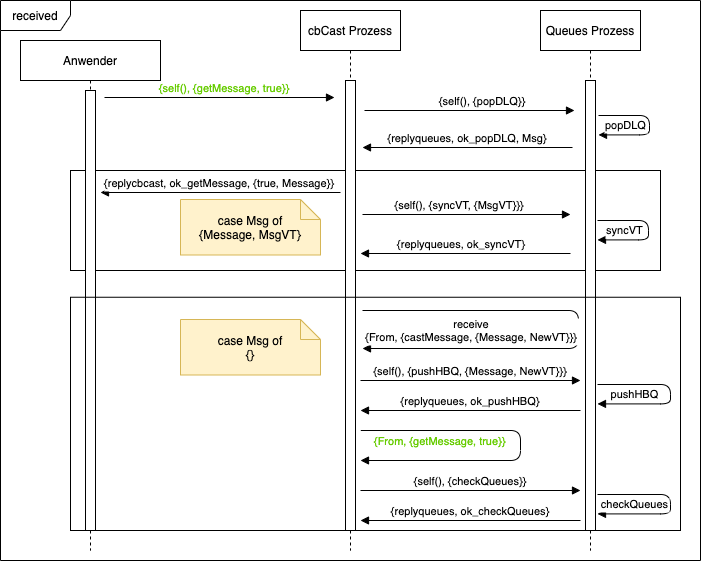
\includegraphics[scale=0.6]{Latex/Bilder/receive_realisierung.png}
\caption{\label{fig:sequence_received_realisierung} received/2}
\end{center}
\end{figure}

\subsubsection{$\{\langle PID \rangle,\{castMessage,\{\langle Message \rangle, \langle VT \rangle\}\}\}$}

Die Schnittstelle \textit{castMessage} (siehe Abb. \ref{fig:sequence_cast_realisierung}) überprüft nach dem Empfangen einer Nachricht ob die Identität der Vektoruhr der Nachricht, die gleiche Identität hat, wie der \textit{Prozess der Kommunikationseinheit}. Wenn dies der Fall ist, wird die Nachricht verworfen, da die Nachricht bereits beim Versenden in der \textit{Delivery Queue} gespeichert wurde.

\begin{figure}[htbp]
\begin{center}
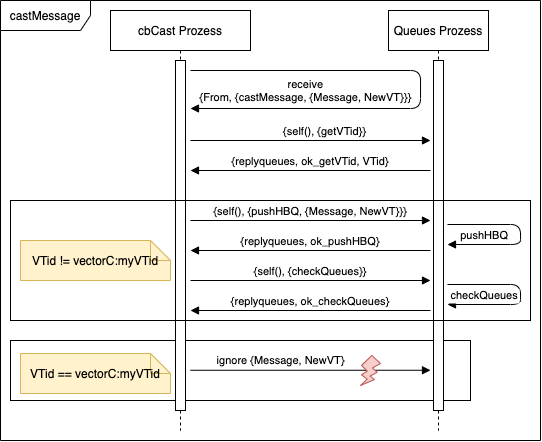
\includegraphics[scale=0.6]{Latex/Bilder/cast_realisierung.png}
\caption{\label{fig:sequence_cast_realisierung} $\{\langle PID \rangle,\{castMessage,\{\langle Message \rangle, \langle VT \rangle\}\}\}$}
\end{center}
\end{figure}

\subsection{Vektoruhr-ADT} \label{vectorC_realisierung}

Die bereits in Kapitel \ref{vectorC_entwurf} beschriebene Datenstruktur ist ein \textit{erlang} Tupel bestehend aus der Vektoruhr Identität als Integer und der Vektoruhr als \textit{erlang} Liste. Ein Beispiel $\{2, [1,3,4,2]\}$. Die Vektoruhr Identität ist $2$ und die Vektoruhr ist $[1,3,4,2]$. Die Identitäten beginnen bei 1. Somit ist die eigene Identität dieser ADT $3$.

\begin{lstlisting}
VT = {2, [1,3,4,2]}.
vectorC:myCount(VT).
3
\end{lstlisting}

\subsubsection{initVT/0}

Diese Funktion stellt im ersten Schritt eine Verbindung zur \textit{TowerClock} über die \textit{erlang} Funktion \textit{net\_adm:ping/1} her. Ist der Verbindungsaufbau erfolgreich, wird am \textit{TowerClock} die Identität angefragt. Zurückgegeben wird diese Identität \textit{VecID} als Tupel \textit{\{VecID, zeros(VecID)\}}. \textit{zeros/1} erstellt eine Liste, welche genau so viele Nullen enthält, wie es im Parameter übergeben wurde.

\subsubsection{myCount/1}

Über die Hilfsfunktion \textit{getElementByIndex(VT, VTID)} kann der entsprechende Ereigniszähler, bzw. der eigene Zeitstempel gefunden werden.

\subsubsection{foCount/2}

\textit{foCount/2} wirft eine Exception, wenn die übergebene Position J kleiner als 0 oder größer als die Länge der verfügbaren Zeitstempel ist.

\begin{lstlisting}
foCount(J, {_VTID, VT}) when J > 0 andalso J =< length(VT)-> getElementByIndex(VT, J);
foCount(_, _) -> throw({error, "Invalid index. Index must be greater than 0 and smaller than the size of available timestamps."}).
\end{lstlisting}

\subsubsection{isVT/1}

Zuerst wird geprüft ob das Tupel genau zwei Elemente enthält. Trifft dies zu, wird geprüft, dass
\begin{enumerate}
    \item das erste Element ein Integer ist,
    \item das zweite Element eine Liste ist,
    \item jedes Element der Liste ein Integer ist.
\end{enumerate}

\subsubsection{syncVT/2} \label{syncVT_realisierung}

Im ersten Schritt dieser Funktion wird zuerst die Länge der beiden übergebenen Vektoruhren anhand der Hilfsfunktion \textit{padWithZeros/2} normalisiert:

\begin{lstlisting}
NormalizedVT1 = padWithZeros(VT1, length(VT2)),
NormalizedVT2 = padWithZeros(VT2, length(VT1)),
\end{lstlisting}

Diese beiden Vektoruhren werden dann Index für Index miteinander verglichen. Es wird jeweils das Maximum der beiden Werte als neue Liste gespeichert und zusammen mit der Identität der ersten Vektoruhr zurückgegeben.

\subsubsection{tickVT/1}

\textit{tickVT/1} nutzt die Hilfsfunktion \textit{incrementElementAtIndex/3}. Übergeben werden dieser Funktion die Vektoruhr an sich, die Identität und ein Counter.

\subsubsection{compVT/2}

Auch in \textit{compVT/2} werden zuerst die beiden Vektoruhren normalisiert (siehe Kapitel \ref{syncVT_realisierung}). 
Anschließend wird die Hilfsfunktion \textit{compareLists/3} (siehe Abb. \ref{fig:flow_compVT_realisierung}) aufgerufen.

\begin{figure}[htbp]
\begin{center}
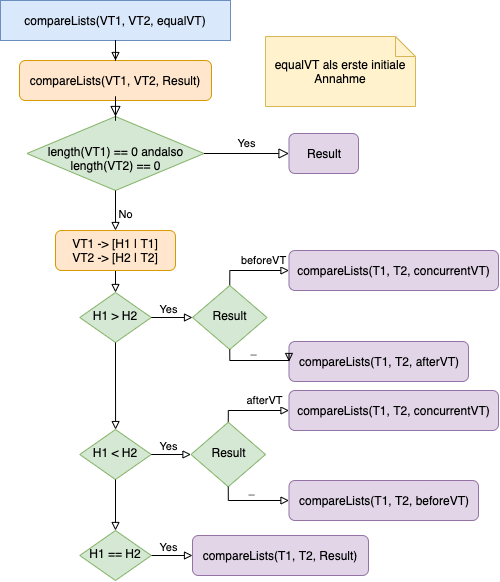
\includegraphics[scale=0.6]{Latex/Bilder/compVT_realisierung.png}
\caption{\label{fig:flow_compVT_realisierung} compVT}
\end{center}
\end{figure}

\subsubsection{aftereqVTJ/2}

Die Funktion \textit{aftereqVTJ/2} (siehe Abb. \ref{fig:flow_aftereqvtj_realisierung}) nutzt zwei weitere Funktionen. Zuerst die \textit{removeJ/2} Hilfsfunktion, welche in beiden Vektoruhren ein Element entfernt und dann die beiden neuen Vektoruhren vergleicht (siehe Kapitel \ref{aftereqvtj_entwurf}).

\begin{figure}[htbp]
\begin{center}
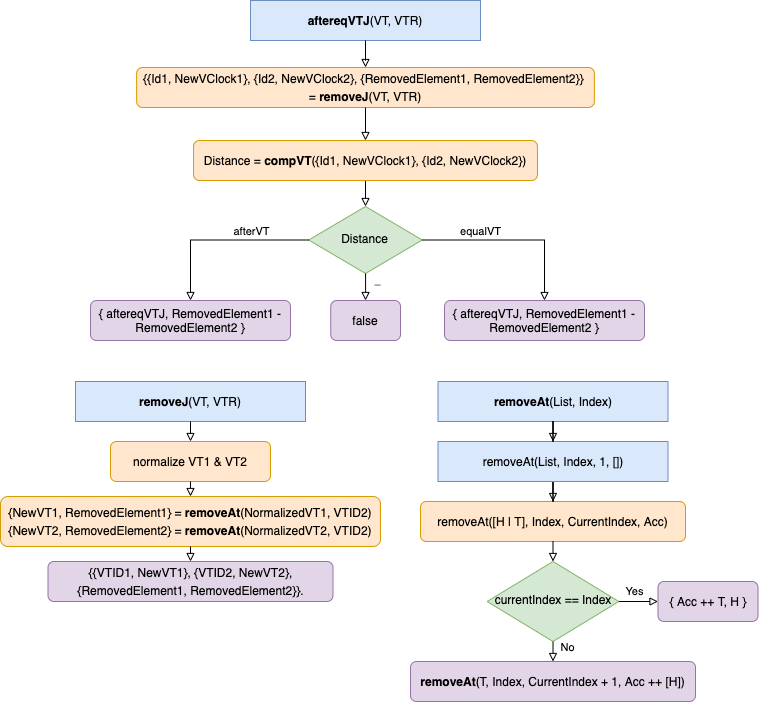
\includegraphics[scale=0.55]{Latex/Bilder/aftereqVTJ_realisierung.png}
\caption{\label{fig:flow_aftereqvtj_realisierung} aftereqVTJ/2}
\end{center}
\end{figure}

\subsection{Ungeordneter Multicast}

\subsubsection{init/1}

\subsubsection{stop/1}

\subsubsection{listall/0}

\subsubsection{cbcast/2}

\subsubsection{$\{\langle PID \rangle,\{register,\langle RPID\rangle\}\}$}

\subsubsection{$\{\langle PID\rangle,\{multicastB,\{\langle Message\rangle,\langle VT\rangle\}\}\}$}

\subsubsection{$\{\langle PID\rangle,\{multicastNB,\{\langle Message\rangle,\langle VT\rangle\}\}\}$}

\subsubsection{$\{\langle PID\rangle,\{multicastM,\langle CommNR\rangle,\langle MessageNR\rangle\}\}$}


\subsection{Vektoruhr Zentrale/Tower}

Aufgabe der \textit{Vektoruhr Zentrale} ist, allen \textit{Prozessen der Kommunikationseinheiten} eine eindeutige Identität zu geben. Diese ist vom Typ Integer und startet bei 1.

\subsubsection{init/0}

Diese Funktion erzeugt einen Prozess, welcher unter der Prozess ID \textit{vtKLCclockC} registriert wird. Der erzeugte Prozess sieht wie folgt aus:

\begin{lstlisting}
loop(Datei, Map) ->
    receive
        {getVecID, PID} ->
            ...
            loop(...
        {From, {stop}} when is_pid(From)->
            ...
        Any -> 
            util:logging(Datei, "Unknown message: "++util:to_String(Any)++"\n"),
            loop(Datei, Map)
    end.
\end{lstlisting}

Gespeichert wird einmal die in die zu loggende Datei und eine Map. Die Map ist als Liste implementiert, welche Objekte enthält. Diese haben alle ein Key Value Paar. Die Keys sind Prozess IDs, die Values sind Integer.

\subsubsection{stop/1}

Das Stoppen des Prozesses funktioniert wie in Kapitel \ref{cbcast_stop_realisierung}.

\subsubsection{$\{getVecID,\langle PID\rangle\}$}

Diese Schnittstelle empfängt eine Prozess ID. Anschließend wird überprüft ob in der Map des Prozesses bereits ein Objekt mit einer solchen Prozess ID gespeichert ist. Wenn ja, wird die zugehörige Identität zurückgeschickt. Ansonsten wird eine neue Identität erzeugt, mit der Prozess ID zusammen in der Map gespeichert und zurückgeschickt. Diese neue Identität berechnet sich durch $length(Map) + 1$.
\section{Analyse} \label{analyse}

\subsection{Korrektheitsbeweis}

\subsection{Komplexitätsanalyse}
\section{Fazit}

% \endgroup

\newpage

\section*{Selbstständigkeitserklärung}

Hiermit erkläre ich, dass ich diese schriftliche Ausarbeitung meiner Hausarbeit selbstständig und ohne fremde Hilfe verfasst habe und keine anderen als die angegebenen Quellen und Hilfsmittel benutzt habe sowie die aus fremden Quellen (dazu zählen auch Internetquellen) direkt oder indirekt übernommenen Gedanken oder Wortlaute als solche kenntlich gemacht habe. Zudem erkläre ich, dass der zugehörige Programmcode von mir selbständig implementiert wurde ohne diesen oder Teile davon von Dritten im Wortlaut oder dem Sinn nach übernommen zu haben. Die Arbeit habe ich bisher keinem anderen Prüfungsamt in gleicher oder vergleichbarer Form vorgelegt. Sie wurde bisher nicht veröffentlicht.\\

\vspace{1cm}
\parbox{4cm}{%
\rule{4cm}{0.5pt}\\
\centerline{(Ort, Datum)}%
}\hfill
\parbox{5cm}{%
\rule{5cm}{0.5pt}\\
\centerline{(Unterschrift)}%
}

\newpage
\addcontentsline{toc}{section}{Abbildungsverzeichnis}
\listoffigures

\addcontentsline{toc}{section}{Literaturverzeichnis}
\printbibliography[title={Literaturverzeichnis}]

\newpage

\end{document}